\documentclass[11pt]{article} % use larger type; default would be 10pt
\usepackage[utf8]{inputenc} % set input encoding (not needed with XeLaTeX)
\usepackage{fullpage}
\usepackage{graphicx} % support the \includegraphics command and options
\usepackage{caption}
\usepackage{subcaption}
\usepackage{amsmath}
\usepackage{amssymb}
\newcommand{\drv}[2]{\ensuremath{\frac{d #1}{d #2}}}
\newcommand{\ddrv}[2]{\ensuremath{\frac{d^2 #1}{d^2 #2}}}
\newcommand{\into}{\ensuremath{\int_{-1}^1}}
\newcommand{\intz}{\ensuremath{\int_0^1}}
\newcommand{\intf}{\ensuremath{\int_{-\infty}^\infty}}
\newcommand{\inti}{\ensuremath{\int_{x_{i-1/2}}^{x_{i+1/2}}}}
\newcommand{\intO}{\ensuremath{\int_{4\pi}}}
\newcommand{\order}[1]{\ensuremath{\mathcal{O}(#1)}}
\newcommand{\He}{\ensuremath{\mbox{He}}}
\newcommand{\expv}[1]{\ensuremath{\langle #1 \rangle}}

\title{Simple problem testing}
\author{Paul Talbot}
%\date{}

\begin{document}
\maketitle

Equation to solve:
\begin{equation}
-D\ddrv{\phi}{x}+\Sigma_a\phi = S,
\end{equation}
\begin{equation}
\phi(x)=\frac{S}{\Sigma_a}\left(1-e^{-x/L}\right),
\end{equation}
\begin{equation}
L^2\equiv \frac{D}{\Sigma_a}.
\end{equation}

\section{Uniform}
We allow $\Sigma_a$ to vary uniformly on $\Sigma_a\in(0.5,1)$ and quantify the uncertainty using stochastic collocation for generalized polynomial expansion as well as Monte Carlo sampling.

For increasing orders of expansion, the mean and variance obtained are shown along with the run time.  The other parameters for $\phi$ are taken as follows:
\begin{align}
S &= 1.0 \text{ n/cm}^2\text{/s},\\
D &= 0.5 \text{ /cm},\\
x &= 2.0 \text{ cm}.
\end{align}
\begin{table}
\begin{center}
\begin{tabular}{c c|l l| r}
type & runs/order & mean & variance & run time (sec) \\ \hline
MC & 23400 & 1.25554670335 & 0.0492854851117 & 742.441\\
SC & 2 & 1.25472215220 & 0 & 2.738\\
SC & 4 & 1.25569029702 & 0.049198975952 & 2.692\\
SC & 8 & 1.25569096924 & 0.0492316191443 & 3.854\\
SC & 16 & 1.25569096924 & 0.0492316191611 & 6.107
\end{tabular}
\end{center}
\caption{Uniform Uncertainty Means, Variances}
\end{table}

The PDFs were obtained by Monte Carlo sampling of the polynomial expansion for the SC cases, and obtained directly for the Monte Carlo case, shown in Fig. \ref{uni}.  The x-axis is the value of the scalar flux, and the y-axis is the probability of obtaining a particular flux.
\begin{figure}[h!]
\centering
   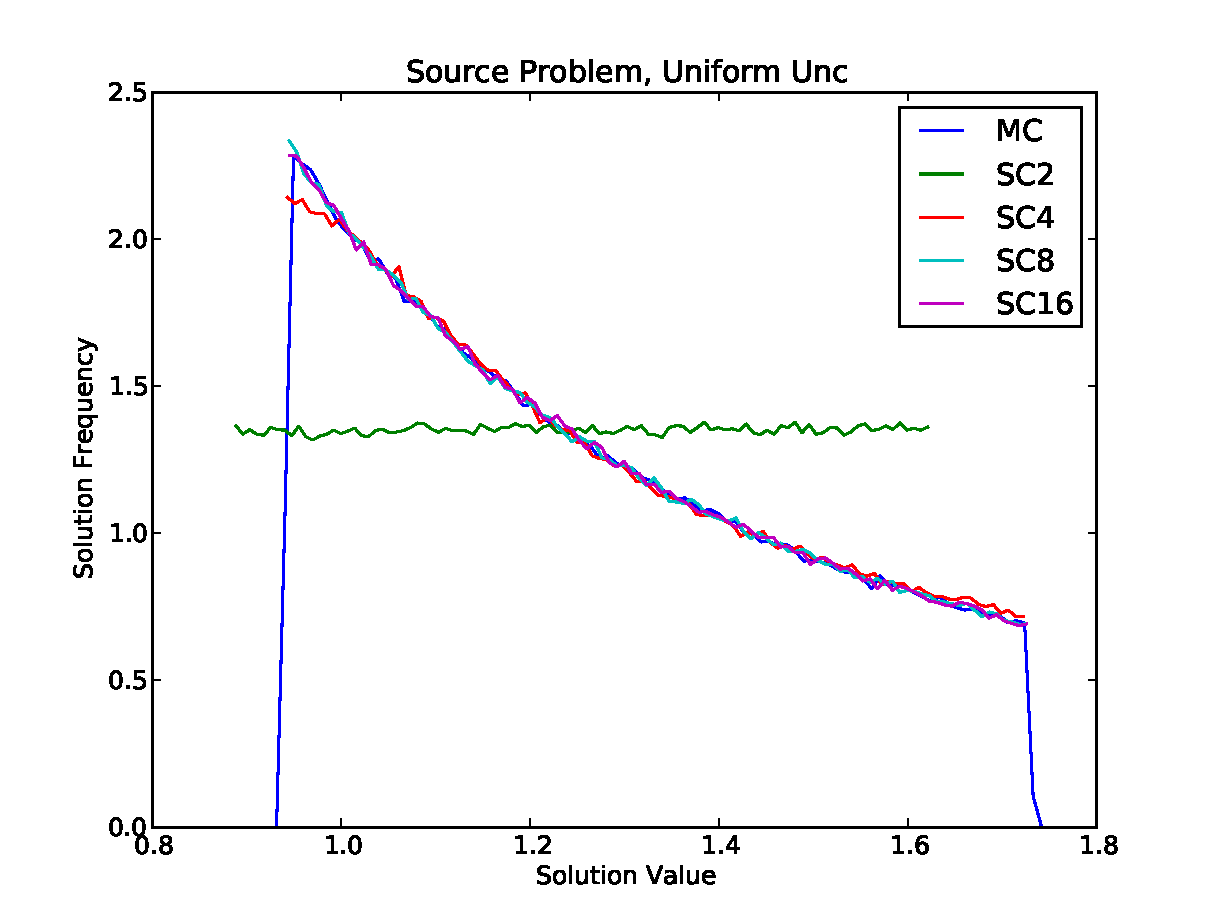
\includegraphics[width=\textwidth]{../graphics/source_uniform_pdfs}
   \label{uni}
   \caption{Uniform PDFs}
\end{figure}


\newpage
\section{Normal}
We allow $\Sigma_a$ to vary uniformly on $\Sigma_a\in\mathcal{N}(0.75,0.15)$ and quantify the uncertainty using stochastic collocation for generalized polynomial expansion as well as Monte Carlo sampling.

For increasing orders of expansion, the mean and variance obtained are shown along with the run time.  The other parameters for $\phi$ are taken as follows:
\begin{align}
S &= 1.0 \text{ n/cm}^2\text{/s},\\
D &= 0.5 \text{ /cm},\\
x &= 2.0 \text{ cm}.
\end{align}
\begin{table}[h!]
\begin{center}
\begin{tabular}{c c|l l| r}
type & runs/order & mean & variance & run time (sec) \\ \hline
MC & 23400 & 1.24922240195 & 0.0488719424418 & 366.31\\
SC & 2 & 1.2547221522 & 0 & 2.08 \\
SC & 4 & 1.25569029702 & 0.049198975952 & 3.11 \\
SC & 8 & 1.25569096924 & 0.0492316191443 & 4.74\\
SC & 16 & 1.25569096924 & 0.0492316191611 & 6.88
\end{tabular}
\end{center}
\caption{Normal Uncertainty Means, Variances}
\end{table}

\begin{figure}[h!]
\centering
   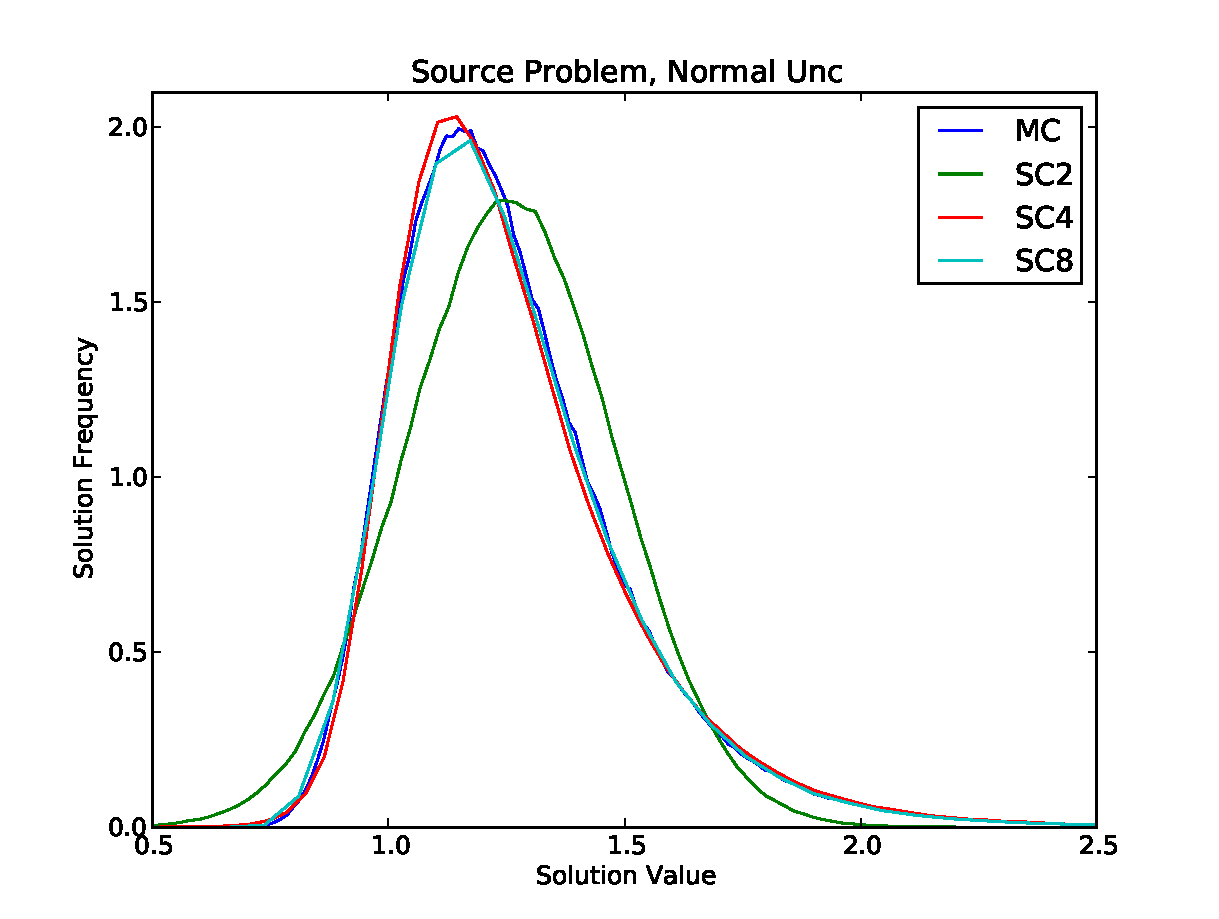
\includegraphics[width=\textwidth]{../graphics/source_normal_pdfs}
   \label{norm}
   \caption{Normal PDFs}
\end{figure}




\end{document}


\begin{center}
\begin{tabular}{c c|c c| c}
\end{tabular}
\end{center}

\begin{figure}[h]
\centering
  \begin{subfigure}[b]{0.45 \textwidth}
   \includegraphics[width=\textwidth]{}
   \caption{}
   \label{}
  \end{subfigure}
  \begin{subfigure}[b]{0.45\textwidth}
   \includegraphics[width=\textwidth]{}
   \caption{}
   \label{}
  \end{subfigure}
\caption{}
\end{figure}